\documentclass{article}
\usepackage[final]{neurips_2026}
\usepackage[utf8]{inputenc} % allow utf-8 input
\usepackage[T1]{fontenc}    % use 8-bit T1 fonts
\usepackage{hyperref}       % hyperlinks
\usepackage{url}            % simple URL typesetting
\usepackage{booktabs}       % professional-quality tables
\usepackage{amsfonts}       % blackboard math symbols
\usepackage{nicefrac}       % compact symbols for 1/2, etc.
\usepackage{microtype}      % microtypography
\usepackage{xcolor}         % colors
\usepackage{graphicx}
\usepackage{float}
\usepackage{amsmath}
\usepackage{algorithm} 
\usepackage{algorithmic}
\usepackage{float}
\usepackage{graphicx}
\raggedbottom

\title{Data Pilot AI Pro - Intelligent Data Analysis Platform}


\author{%
  Bhavana Vippala \\
  MS in Data Science\\
  University of Colorado Boulder\\
  \texttt{bhvi9697@colorado.edu} \\
  % examples of more authors
  \And
  Shivaraj Senthil Rajan \\
  MS in Data Science\\
  University of Colorado Boulder\\
  \texttt{shse1502@colorado.edu} \\
  \And
  Manohar Korikana \\
  MS in Data Science\\
  University of Colorado Boulder\\
  \texttt{mako6854@colorado.edu}
  \And
  Harshitha Attanti \\
  MS in Data Science\\
  University of Colorado Boulder\\
  \texttt{haat9091@colorado.edu}
  % \AND
  % Coauthor \\
  % Affiliation \\
  % Address \\
  % \texttt{email} \\
  % \And
  % Coauthor \\
  % Affiliation \\
  % Address \\
  % \texttt{email} \\
  % \And
  % Coauthor \\
  % Affiliation \\
  % Address \\
  % \texttt{email} \\
}


\begin{document}


\maketitle

\thispagestyle{plain}
\pagestyle{plain}
\pagenumbering{arabic}

\begin{abstract}
The ability to extract actionable knowledge from data has become essential across industries, yet the process of building machine learning models and generating meaningful insights remains largely confined to those with deep technical expertise. This creates a significant gap between the organizations that collect data and those that can actually leverage it for decision making. In this paper, we introduce Data Pilot AI Pro, an autonomous data science platform designed to bridge this gap by enabling users, regardless of their technical background, to go from a raw dataset to trained models, interpretable predictions, and business outcomes without writing a single line of code. The system orchestrates seven specialized agents that collaboratively handle every stage of the data science workflow, from profiling and cleaning through feature engineering, model training, visualization, and explainability. Central to our approach is a reinforcement learning agent trained with Proximal Policy Optimization model on diverse real world datasets sourced from OpenML, which learns to recommend the most effective algorithm for a given dataset by analyzing its underlying statistical characteristics. To ensure transparency, model predictions are accompanied by SHAP and LIME explanations enriched with plain language narratives generated by a large language model, making the reasoning behind every prediction understandable to a non-technical audience. For business stakeholders, the platform further offers an intelligent analysis mode that autonomously discovers patterns in the data and presents them as interactive dashboards with natural language summaries. Our evaluation demonstrates that the platform consistently delivers competitive model performance while making the full power of data science accessible to data scientists, business managers, and decision makers alike.

\end{abstract}




\section{Introduction}

Consider a small business owner with years of sales data in spreadsheets but no data science team, or a hospital administrator who needs to predict patient readmission risks without the budget for ML engineers. These are not edge cases but the reality for most organizations, where the gap between having data and being able to use it grows every year. A typical data science workflow involves profiling, cleaning, feature engineering, algorithm selection, model evaluation, and result interpretation, each requiring judgment that even experienced practitioners find time consuming.

Existing AutoML tools such as Auto sklearn, TPOT, and H2O AutoML have automated algorithm selection and hyperparameter optimization, but they assume the user has already prepared a clean, well engineered feature matrix, leaving cleaning and feature engineering (which consume most of a data scientist's effort) to the user. Beyond modeling, their outputs are statistical metrics opaque to non technical stakeholders. What is needed is a unified platform handling the entire journey from raw data to actionable insight.

In this paper we introduce Data Pilot AI Pro, an autonomous end to end data science platform that unifies data preparation, intelligent model selection, training, explainability, and business intelligence into a single coherent system. Seven specialized agents coordinated through a LangGraph orchestrator cover profiling, cleaning, feature engineering, RL guided model training with voting ensembles, interactive visualization, SHAP and LIME explainability with LLM narratives, and autonomous business insight discovery. The model selector at its core is trained with Proximal Policy Optimization on OpenML datasets, learning to map 40 meta features to the most effective algorithm. The platform is deployed as a Streamlit application where a user uploads a CSV and receives trained models, explanations, and dashboards within minutes, requiring no code.

Our contributions are fourfold: (1) a fully automated pipeline covering every stage from raw data to explainability; (2) a PPO based RL model selector trained on OpenML data; (3) a bridge between technical outputs and business understanding via SHAP and LIME with LLM narratives plus an autonomous data analysis mode; and (4) a modular LangGraph architecture where individual agents can be improved or replaced independently.




\subsection{Related Work}

AutoML has been an active research area for over a decade, beginning with Auto WEKA \citep{thornton2013auto}, Auto sklearn \citep{feurer2015efficient}, and TPOT \citep{olson2016tpot}, with commercial platforms like H2O AutoML, Google AutoML, and Amazon SageMaker Autopilot bringing these ideas to production. All share a common limitation: they focus on the modeling stage and assume the user has already prepared clean, well engineered data. The Algorithm Selection Problem \citep{rice1976algorithm}, studied through StatLog and OpenML \citep{vanschoren2014openml}, shows dataset meta features can predict which algorithm performs best, but traditional meta learning relies on static mappings that struggle with complex nonlinear relationships. Our work frames model selection as a reinforcement learning problem where a PPO agent learns a dynamic policy, while also automating stages before and after training that existing AutoML tools leave to the user.

Explainability methods SHAP \citep{lundberg2017unified} and LIME \citep{ribeiro2016lime} are now standard, but their outputs are numerical scores and coefficient tables that non technical stakeholders find hard to interpret. LLM based tools like ChatGPT Code Interpreter and Pandas AI lower the barrier to data exploration but are reactive and require users to know what to ask. We address both gaps by using an LLM to translate SHAP and LIME into plain language narratives, and by providing a proactive Data Analyzer agent that autonomously generates dashboards.

Recent LLM agent systems such as DS Agent \citep{guo2024dsagent} and Data Interpreter \citep{Hong2024data} rely entirely on the LLM to generate and execute code at every step, making them susceptible to hallucination on computationally intensive operations. Data Pilot AI Pro takes a hybrid approach: deterministic expert coded agents handle critical stages like cleaning, feature engineering, and model training, while LLM powered agents handle contextual reasoning tasks like insight discovery and narrative explanation.




\section{Learning and Project Goals}

The gaps in existing work motivated a focused set of learning objectives. Our primary goal was to understand how reinforcement learning can be applied to a real world decision making problem outside its traditional domains of game playing and robotics, specifically how to design a custom Gymnasium environment, define meaningful rewards from model performance, and train a PPO agent that generalizes to unseen datasets. Equally important was learning how LLMs can be embedded in structured pipelines as reasoning components at specific stages rather than as standalone conversational tools, and understanding where LLMs outperform deterministic code versus where they do not. We also aimed to develop end to end understanding of the machine learning lifecycle, particularly profiling, cleaning, and feature engineering which dominate real world practice but are often glossed over in coursework. Finally, we wanted hands-on experience designing multi-agent architectures with LangGraph.





\section{Background}

\subsection{Theory}

The theoretical foundation of Data Pilot AI Pro rests on several
interconnected pillars, the most important of which is reinforcement
learning with Proximal Policy Optimization, the core of our automated model
selection. Our setup is a \emph{contextual bandit}: each episode consists of
one step where the agent observes a dataset meta-feature vector, selects an
algorithm, and receives a reward from its hold-out performance, with no
temporal dependencies between datasets. Formally the problem is the tuple
$(\mathcal{S}, \mathcal{A}, R)$, where $\mathcal{S} \subseteq [0,1]^{40}$ is
the space of normalized meta-feature vectors, $\mathcal{A}$ is the finite
action set ($|\mathcal{A}| = 8$ for classification, $9$ for regression),
and $R(s, a)$ is rank normalized so the best algorithm scores $1.0$ and the
worst $0.0$ (defined precisely in Section~4.10). The agent learns a policy
$\pi_\theta(a \mid s)$ that maximizes expected reward:

\begin{equation}
    J(\pi) = \mathbb{E}_{s \sim \mathcal{D}}\!\Big[R\!\big(s,\; a\big)\Big],
    \quad a \sim \pi_\theta(\cdot \mid s)
    \label{eq:objective}
\end{equation}

We use PPO \citep{schulman2017proximal} rather than simpler bandit algorithms
because its clipped surrogate objective handles noisy cross-validation
rewards stably and the Stable Baselines3 implementation supports categorical
actions out of the box.


Policy gradient methods directly optimize the policy by computing gradients
of the expected reward with respect to the policy parameters. The policy
gradient theorem \citep{sutton1999policy} expresses the gradient of the
expected return $J(\theta)$ as:

\begin{equation}
\nabla_\theta J(\theta) = \mathbb{E}\left[\nabla_\theta \log \pi_\theta(a \mid s) \, A(s, a)\right]
\end{equation}

where $A(s, a) = Q(s, a) - V(s)$ is the advantage function estimated in
practice using Generalized Advantage Estimation \citep{schulman2016gae}.
Vanilla policy gradient methods can collapse when large updates push the
policy outside the region where the gradient estimate remains accurate,
which motivated trust region methods such as TRPO \citep{schulman2015trust}
and its simpler successor Proximal Policy Optimization.

PPO \citep{schulman2017proximal} achieves trust region stability with a
simpler clipped surrogate objective. Let $r_t(\theta)$ denote the
probability ratio between the new and old policies:

\begin{equation}
r_t(\theta) = \frac{\pi_\theta(a_t \mid s_t)}{\pi_{\theta_{\text{old}}}(a_t \mid s_t)}
\end{equation}

The PPO objective is then:

\begin{equation}
L^{\text{CLIP}}(\theta) = \mathbb{E}_t\left[\min\left(r_t(\theta) \, \hat{A}_t, \; \text{clip}\left(r_t(\theta), \, 1 - \epsilon, \, 1 + \epsilon\right) \hat{A}_t\right)\right]
\end{equation}

where $\epsilon$ (typically $0.2$) bounds the maximum deviation. The clip
prevents runaway updates in either direction: when the advantage is
positive the ratio cannot exceed $1 + \epsilon$, and when negative it
cannot fall below $1 - \epsilon$. This simple clipping empirically matches
the more expensive KL constraints of TRPO.

The second theoretical pillar underlying our system is the framework of model 
explainability through SHAP, which is grounded in the theory of Shapley values 
from cooperative game theory \citep{shapley1953value}. In this framework, a 
prediction is treated as a cooperative game where each feature is a player and 
the prediction outcome is the total payout, and the goal is to fairly distribute 
credit for the prediction among all features based on their individual 
contributions. The Shapley value for feature $i$ is formally defined as:

\begin{equation}
\phi_i = \sum_{S \subseteq F \setminus \{i\}} \frac{|S|!\;(|F| - |S| - 1)!}{|F|!} \left[f(S \cup \{i\}) - f(S)\right]
\end{equation}

where $F$ is the full set of features and $f(S)$ is the model's prediction
using only the features in subset $S$. Exact Shapley values require
evaluating the model on all feature subsets and scale exponentially, so SHAP
\citep{lundberg2017unified} uses efficient approximations including TreeSHAP
for tree based models which runs in polynomial time by exploiting the tree
structure.

The third theoretical component is LIME \citep{ribeiro2016lime}, which
explains individual predictions by fitting a simple linear surrogate model in
the local neighborhood of the instance $x$. LIME generates perturbed samples
around $x$, queries the original model, and fits a weighted linear regression
where the sample weights come from an exponential kernel:

\begin{equation}
\pi_x(z) = \exp\left(-\frac{D(x, z)^2}{\sigma^2}\right)
\end{equation}

where $z$ is a perturbed sample, $D(x, z)$ is the distance from the original
instance, and $\sigma$ controls the kernel width. The coefficients of the
resulting sparse linear model indicate how much each feature contributed at
that specific point. The theoretical insight is that while the global
decision boundary of a complex model may be highly nonlinear, in a small
neighborhood it can be well approximated by a linear function. In our
pipeline the LLM then synthesizes both SHAP and LIME outputs into a unified
natural language narrative.

The fourth theoretical pillar of our system is the framework of LLM agents and
tool calling, which underlies our decision to build Data Pilot AI Pro as a
collection of seven specialized agents rather than a single end to end model.
Unlike the previous three pillars, this area is relatively new and does not yet
have a clean closed form mathematical theory, so we ground our design in
empirical findings from recent research that consistently point in the same
direction.

A large language model on its own is good at reading instructions and producing
text, but it is not reliable at doing math, running code, or remembering long
chains of facts without making mistakes. Tool calling solves this by letting
the model decide what to do and then handing the actual computation to an
external tool that is guaranteed to be correct. The model writes a small
structured request such as ``run cross validation with 5 folds on this dataset'',
the request is executed by trusted code, and the numerical result is returned
to the model so it can continue reasoning. Empirical work such as ReAct
\citep{yao2023react} and Toolformer \citep{schick2023toolformer} has shown
that this pattern produces noticeably more accurate answers on tasks
involving numbers, lookups, or multi step planning. In our pipeline we
apply the same idea: each agent uses the LLM only for parts that benefit
from language understanding, while imputation, encoding, cross validation,
SHAP, and LIME are delegated to deterministic libraries.

The second question is why seven separate agents instead of one. A single
prompt asked to profile, clean, engineer features, train, explain, and
visualize must hold all of that context at once, and empirical multi agent
systems show this hurts reliability. AutoGen \citep{wu2024autogen} reports
that specialized agent conversations outperform a single agent on math,
coding, and decision making benchmarks; ChatDev \citep{qian2024chatdev}
finds similar gains when software engineering is split across role based
agents; and DS Agent \citep{guo2024dsagent} and Data Interpreter
\citep{Hong2024data} extend the pattern to data science and observe fewer
hallucinations with sub agents than with a monolithic prompt. Our own early
prototype that used one LLM call for the entire pipeline produced unstable
code, and moving to seven focused agents eliminated most of these problems.

\begin{table}[h]
\centering
\caption{Summary of key mathematical notation used in this work}
\begin{tabular}{@{}ll@{}}
\toprule
\textbf{Symbol} & \textbf{Description} \\
\midrule
$(S, A, P, R, \gamma)$ & Markov Decision Process tuple \\
$\pi_\theta(a \mid s)$ & Policy parameterized by $\theta$ \\
$J(\pi)$ & Expected cumulative discounted reward (Eq. 1) \\
$A(s, a)$ & Advantage function (Eq. 3) \\
$Q(s, a)$ & Action-value function \\
$V(s)$ & State-value function \\
$r_t(\theta)$ & Probability ratio, new policy / old policy (Eq. 4) \\
$L^{\text{CLIP}}(\theta)$ & PPO clipped surrogate objective (Eq. 5) \\
$\epsilon$ & PPO clipping parameter (default $0.2$) \\
$\phi_i$ & Shapley value for feature $i$ (Eq. 6) \\
$F$ & Full set of features \\
$f(S)$ & Model prediction using feature subset $S$ \\
$\pi_x(z)$ & LIME locality kernel weight (Eq. 7) \\
$D(x, z)$ & Distance between instance and perturbation \\
\bottomrule
\end{tabular}
\end{table}

\section{Method}

Having established the theoretical foundations in the previous section, we now 
describe the design and implementation of Data Pilot AI Pro in sufficient detail 
that the system could be reproduced independently. The platform is built as a 
modular multi agent pipeline where each stage of the data science workflow is 
handled by a specialized agent, and a central orchestrator coordinates their 
execution through a directed acyclic graph with shared state.

\subsection{System Architecture}

The architecture of Data Pilot AI Pro follows a pipeline pattern coordinated by 
a LangGraph StateGraph that defines the execution order and conditional routing 
between seven specialized agents. The entire system state is represented as a 
single shared dictionary that flows through each agent in sequence, with every 
agent reading the outputs of its predecessors and appending its own results. 
The orchestrator supports three execution modes: in ML Pipeline mode, data 
flows through Context Analyzer, Profiler, Cleaner, Feature Engineer, Modeler, 
Visualizer, and Explainer in sequence; in Data Analysis mode, data is routed 
directly to the Data Analyzer; and in Combined mode, the full ML pipeline 
executes first followed by the Data Analyzer.

% Replace with actual diagram file when ready
\begin{figure}[H]
\centering
\includegraphics[width=0.95\textwidth]{figures/system architecture.jpeg}
\caption{System architecture of Data Pilot AI Pro showing the LangGraph orchestrator routing data through two execution modes: Tab 1 (Data Insights) for LLM-powered dashboard generation, and Tab 2 (Data Pipeline) for the full 8-stage ML pipeline from context analysis through post-deployment prediction.}
\label{fig:architecture}
\end{figure}


To make the orchestration concrete, Algorithm~\ref{alg:pipeline} formalizes the end-to-end flow that DataPilot AI Pro executes on every user request. 




\begin{algorithm}[H]
\caption{Data Pilot AI Pro: End-to-End Pipeline Orchestration}
\label{alg:pipeline}
\begin{algorithmic}[1]
\REQUIRE Dataset $\mathcal{D}$, target column $t$, execution mode $m \in \{\text{ML}, \text{Analysis}, \text{Combined}\}$
\ENSURE Trained model $\mathcal{M}^*$, explanations $\mathcal{E}$, insights $\mathcal{I}$, visualizations $\mathcal{V}$
\STATE $\mathcal{S} \leftarrow \text{InitializeState}(\mathcal{D}, t, m)$
\STATE \textit{// Stage 1: Context Analysis and Profiling}
\STATE $\mathcal{S} \leftarrow \text{ContextAgent.execute}(\mathcal{S})$ \COMMENT{Detect task type, column roles}
\STATE $\mathcal{S} \leftarrow \text{ProfilerAgent.execute}(\mathcal{S})$ \COMMENT{Extract 40 meta-features $\mathbf{f} \in [0,1]^{40}$}
\IF{$m = \text{Analysis}$}
    \STATE $\mathcal{I} \leftarrow \text{DataAnalyzer.execute}(\mathcal{S})$
    \RETURN $\mathcal{I}$
\ENDIF
\STATE \textit{// Stage 2: Data Preprocessing}
\STATE $\mathcal{S} \leftarrow \text{CleanerAgent.execute}(\mathcal{S})$ \COMMENT{Impute, remove outliers, fix types}
\STATE $\mathcal{S} \leftarrow \text{FeatureAgent.execute}(\mathcal{S})$ \COMMENT{Encode, select, scale features}
\STATE \textit{// Stage 3: Model Selection and Training}
\STATE $\mathbf{p} \leftarrow \text{PPO}_\theta(\mathbf{f})$ \COMMENT{RL policy outputs model probabilities}
\STATE $\text{top\_models} \leftarrow \text{argsort}(\mathbf{p})[-3:]$
\FOR{each model $m_i \in \text{top\_models}$}
    \STATE $s_i \leftarrow \text{CrossValidate \& Hyper Parameter tuning}(m_i, \mathcal{D}_{\text{processed}}, k=5)$
\ENDFOR
\STATE $\mathcal{M}^* \leftarrow \text{VotingEnsemble}(\text{top\_models}, \text{weights} \propto [s_1, s_2, s_3])$
\STATE \textit{// Stage 4: Explanation and Visualization}
\STATE $\mathcal{E} \leftarrow \text{ExplainerAgent.execute}(\mathcal{S})$ \COMMENT{SHAP + LIME + LLM narratives}
\STATE $\mathcal{V} \leftarrow \text{VisualizerAgent.execute}(\mathcal{S})$ \COMMENT{Interactive Plotly charts}
\IF{$m = \text{Combined}$}
    \STATE $\mathcal{I} \leftarrow \text{DataAnalyzer.execute}(\mathcal{S})$
\ENDIF
\RETURN $\mathcal{M}^*, \mathcal{E}, \mathcal{I}, \mathcal{V}$
\end{algorithmic}
\end{algorithm}


All agents inherit from a shared BaseAgent abstract class that provides an 
\texttt{execute(state)} interface and an \texttt{ask\_llm(prompt)} method for 
accessing the Gemini 2.5 Flash model. Table~\ref{tab:agents} 
summarizes each agent in the pipeline.

\begin{table}[h]
\centering
\caption{Summary of the seven agents in the Data Pilot AI Pro pipeline.}
\label{tab:agents}
\begin{tabular}{@{}llll@{}}
\toprule
\textbf{Agent} & \textbf{Stage} & \textbf{Key Inputs} & \textbf{Key Outputs} \\
\midrule
Context Analyzer & 0 & Raw data & Domain, target suggestion, hints \\
Profiler & 1 & Raw data & Column types, 40 meta features, quality score \\
Cleaner & 2 & Profiled data & Clean data, imputation map, outlier bounds \\
Feature Engineer & 3 & Clean data & Feature matrix $X$, target vector $y$ \\
Modeler & 4 & $X$, $y$, meta features & Trained models, ensemble, CV scores \\
Visualizer & 5 & Full pipeline state & Interactive Plotly charts (HTML) \\
Explainer & 6 & Models, $X$, $y$ & SHAP, LIME, LLM narratives \\
Data Analyzer & Alt & Raw data & Insights, dashboards, summaries \\
\bottomrule
\end{tabular}
\end{table}

\subsection{Context Analyzer: LLM Powered Data Understanding}

Before any statistical processing begins, the Context Analyzer sends the 
dataset's column names, sample rows, and basic statistics to the LLM, which 
returns a structured JSON identifying the business domain, the most likely 
target column, the task type, and specific cleaning hints for columns requiring 
special treatment. This context is consumed by downstream agents: the Profiler 
uses the suggested target, the Cleaner reads cleaning hints, and the Feature 
Engineer uses feature hints. The key design choice is that the LLM provides 
guidance but never overrides deterministic logic, ensuring the system benefits 
from contextual reasoning without depending on it for correctness.

\subsection{Profiler Agent: Data Analysis and Meta Feature Extraction}

The Profiler produces a comprehensive statistical portrait of the dataset by 
detecting the semantic type of each column (numeric, categorical, binary, 
datetime, text, or identifier), auto detecting the target column using a 
priority hierarchy of common naming conventions, and determining the task type 
based on the target's cardinality. It computes per column statistics including 
mean, standard deviation, skewness, kurtosis, and missing value percentages, 
and assigns a data quality score on a 0 to 100 scale with deductions for 
missing values, duplicates, constant columns, and high cardinality strings. 
The Profiler also performs describe based anomaly detection to spot extreme 
outliers and heavy skew, and a uniformity check to detect case inconsistencies 
in categorical columns.

A critical output is the extraction of 40 meta features organized into eight 
groups (basic shape, missing patterns, statistical distributions, categorical 
properties, target characteristics, PCA dimensionality, landmark model scores, 
and signal quality indicators), all normalized to $[0, 1]$ to serve as the 
observation vector for the PPO agent described in the Background section.

\subsection{Cleaner Agent: Automated Data Cleaning}

The Cleaner applies five operations in sequence: duplicate removal, missing
value imputation, outlier handling, data type correction, and category
standardization. Missing value handling adapts to column type and missing
percentage: numeric columns use median or mean imputation below 5\% missing,
KNN imputation with $k=5$ for 5--30\%, and median plus an indicator column
above 30\%; categorical columns use mode imputation below 10\% and a new
``Missing'' category above. Outlier detection uses IQR based Winsorizing
($Q1 - 1.5 \times IQR$ and $Q3 + 1.5 \times IQR$) only when outliers
constitute less than 5\% of the column. The agent also resolves category
inconsistencies like ``Male'', ``male'', and ``MALE'' by selecting the most
frequent variant as canonical.

\subsection{Feature Engineering Agent: Preparing Data for Modeling}

The Feature Engineer transforms cleaned data into a numeric feature matrix
through five operations: dropping non modelable columns (ID, datetime,
text), categorical encoding, feature selection, VIF based multicollinearity
removal, and numerical scaling. Categorical encoding is tiered: label
encoding for binary columns, one hot with the first category dropped for up
to 10 unique values, and target encoding with smoothing for higher
cardinality. When the feature space exceeds 50 dimensions, features above
$0.95$ correlation are dropped first and the remaining are ranked by mutual
information with the top 50 retained. VIF based removal uses
$VIF_j = 1/(1-R^2_j)$ with a threshold of 10; when multiple features exceed
the threshold, the one with the lowest correlation to the target is dropped
to preserve predictive power. Numerical scaling uses RobustScaler when mean
absolute skewness exceeds 1 and StandardScaler otherwise.

\subsection{Modeler Agent: RL Guided Model Selection and Ensemble Training}

The Modeler feeds the 40 meta features through the trained PPO policy to
get a probability distribution over candidate algorithms, and selects the
top 3. The classification pool is LogisticRegression, GaussianNB,
KNeighborsClassifier, SVC, DecisionTreeClassifier, RandomForestClassifier,
ExtraTreesClassifier, and GradientBoostingClassifier; regression uses
Ridge, Lasso, ElasticNet, SVR, KNeighborsRegressor, DecisionTreeRegressor,
RandomForestRegressor, ExtraTreesRegressor, and GradientBoostingRegressor.
Each pick is trained with 5 fold CV, the three are combined into a
VotingClassifier (soft voting) or VotingRegressor, and the system keeps
whichever performs best overall. Post training the agent runs overfitting
detection (flagging scores above $0.98$ or train-CV gaps above $0.05$),
error analysis, and segment analysis across quantile groups of each numeric
column.

\subsection{Visualizer Agent: Interactive Pipeline Visualization}

The Visualizer generates interactive Plotly charts in four groups
corresponding to each pipeline stage: data overview (type distributions,
missing heatmaps, quality gauges), cleaning impact (before/after
comparisons, outlier box plots), feature analysis (correlation heatmaps,
importance rankings, distribution plots), and model performance (CV scores,
ensemble vs individual models, confusion matrices or residual plots).
Charts are saved as standalone HTML files with a consolidated dashboard.

\subsection{Explainer Agent: SHAP, LIME, and LLM Narratives}

The Explainer provides three levels of interpretability. Globally, SHAP
values are computed with TreeExplainer (KernelExplainer as fallback),
producing beeswarm plots, feature importance bars, and interaction plots.
Locally, SHAP waterfall plots and LIME explanations are generated for
representative samples, with LIME using 5000 perturbations and the kernel
from Equation 7. At the narrative level, the LLM receives SHAP rankings,
metrics, and pipeline reports and produces a structured report covering
dataset issues, cleaning rationale, feature engineering impact, model
selection reasoning, and business recommendations. For individual
predictions it translates SHAP and feature values into 2--3 sentence plain
English explanations.

\subsection{Data Analyzer Agent: LLM Powered Business Intelligence}

The Data Analyzer autonomously discovers 6--8 business relevant insights
from any uploaded dataset. It sends column info, sample data, and
statistical highlights to the LLM, which returns a JSON structure
specifying each insight's title, chart type, column mappings, and
aggregation. The agent programmatically generates each Plotly chart and
calls the LLM again for natural language narratives. It also supports
conversational follow up where users type questions and receive dynamically
generated visualizations.

\subsection{RL Model Selector: Training Pipeline}

The RL selector is trained offline by collecting OpenML datasets,
extracting 40 meta-features per dataset, and evaluating all candidate
algorithms with a 75/25 hold-out split to record their actual scores. A
single train-test split is used rather than cross-validation because every
candidate must be evaluated on every training dataset during environment
construction. The resulting data is loaded into a custom Gymnasium
environment where each single-step episode presents a dataset's
meta-features as the observation and the agent selects one of $n$
candidates. The reward is rank based: given action $a$ with hold-out score
$s(a, \mathcal{D})$, its rank is the number of actions with strictly higher
scores:
\begin{equation}
\text{rank}(a) = \left| \{ a' \in \mathcal{A} : s(a', \mathcal{D}) > s(a, \mathcal{D}) \} \right|
\end{equation}
The reward is then normalized to $[0, 1]$ where the best model receives 1.0 
and the worst receives 0.0:
\begin{equation}
r(a, \mathcal{D}) = 1 - \frac{\text{rank}(a)}{n - 1}
\end{equation}
where $n = |\mathcal{A}|$ is the total number of candidate models (8 for 
classification, 9 for regression). This rank-based formulation provides a 
smooth reward signal that encourages the agent to consistently identify 
top-performing models rather than merely favoring any above-average candidate.

The PPO agent uses a 3-layer MLP policy (256, 256, 128 neurons), is trained
for 50,000 to 100,000 timesteps per task type with clipping parameter
$\epsilon = 0.2$, and the trained model is saved as a pickle file for
inference.

\subsection{PPO Policy Network Architecture}

The policy network is a fully connected MLP implemented using Stable
Baselines3's MlpPolicy (Figure~\ref{fig:ppo_network}). It takes the 40
dimensional meta-feature vector, passes it through three hidden layers of
256, 256, and 128 neurons with ReLU activations, and produces a Softmax
probability distribution over the candidate algorithms. Classification has
8 output units, regression has 9. At inference the Modeler extracts the 40
meta-features, runs a single forward pass, and uses the output
probabilities to rank candidates and pick the top 3 for ensemble
construction. The 256-256-128 bottleneck concentrates representational
capacity near the input where feature interactions are complex and narrows
toward the output where only relative weights across a small action set
are needed. Separate networks are trained for classification and
regression because their action spaces differ and joint training was
unstable.

\begin{figure}[H]
\centering
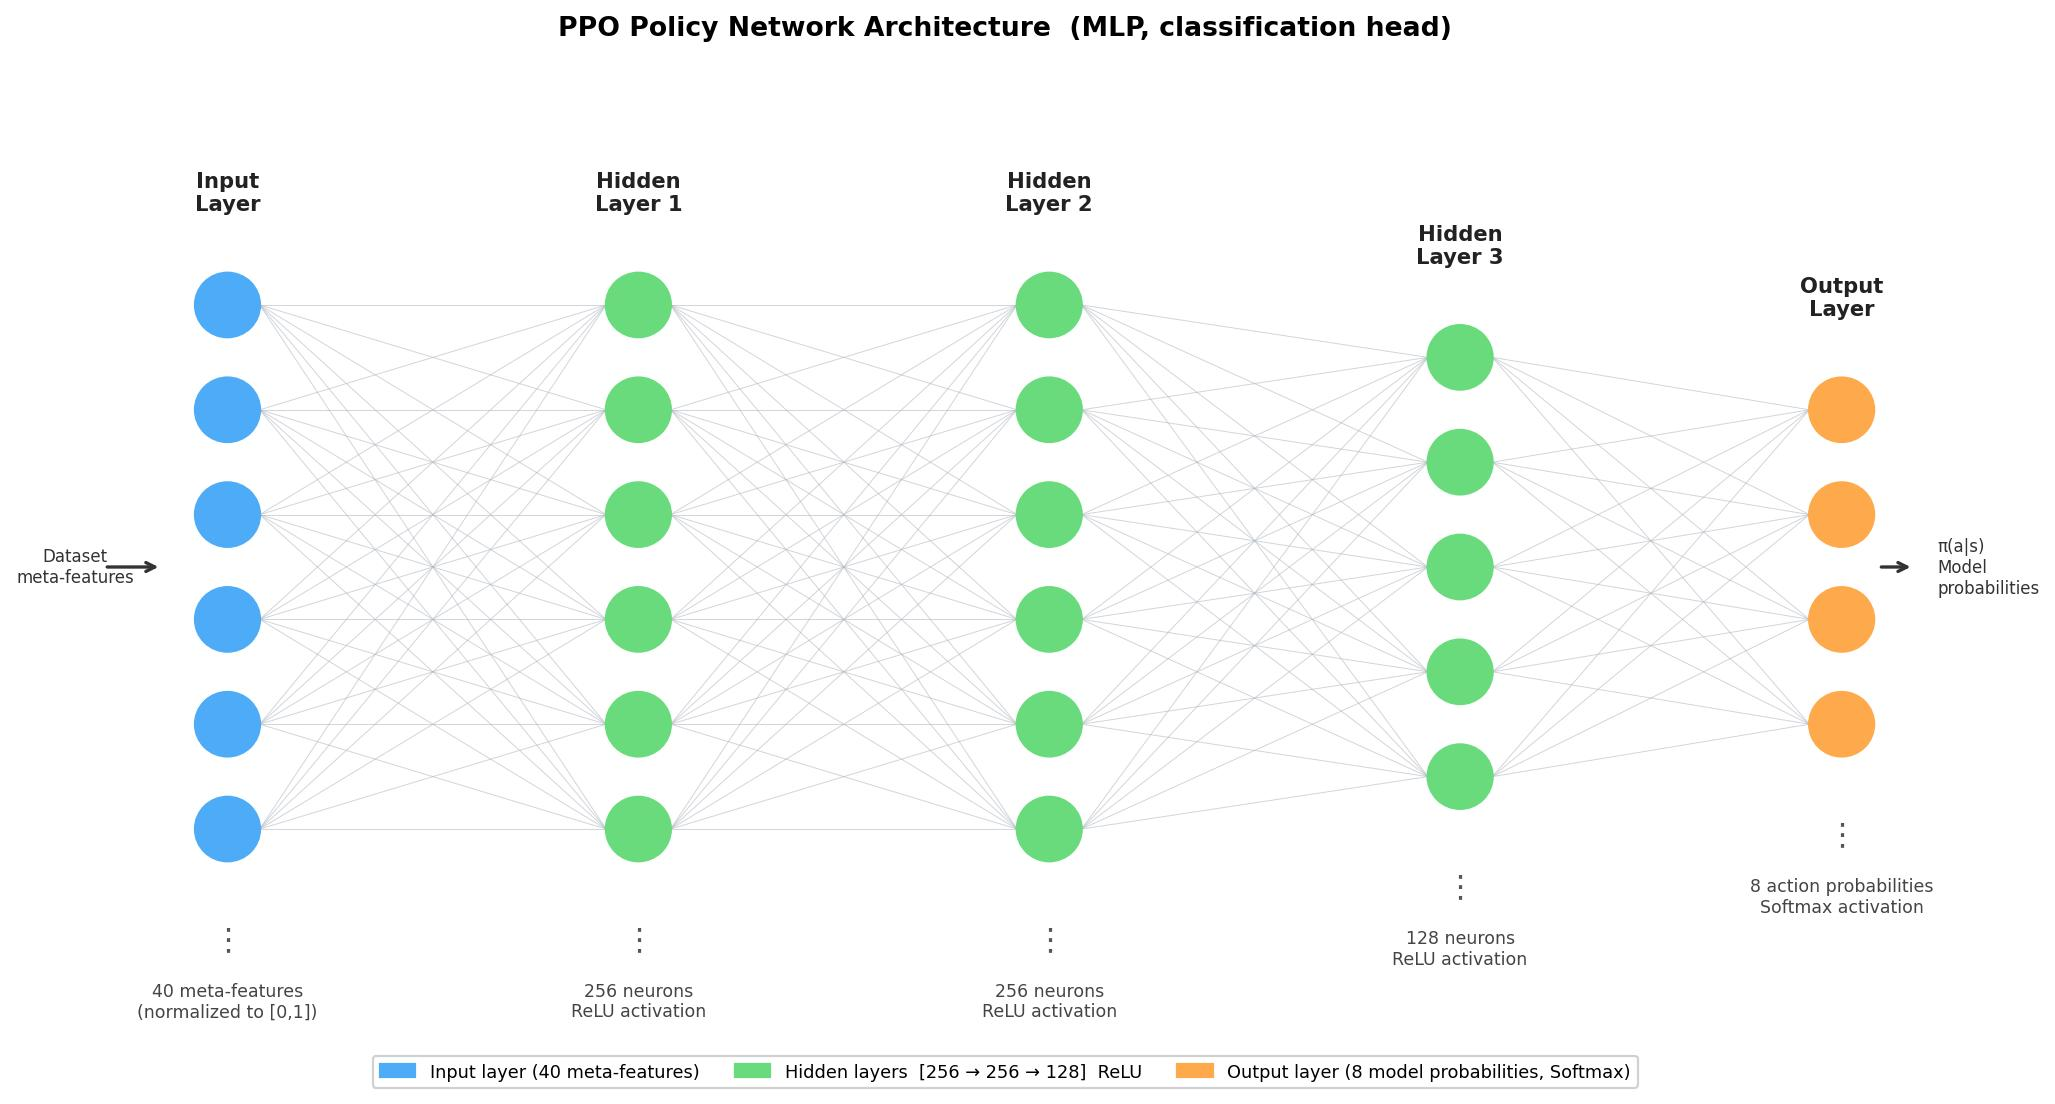
\includegraphics[width=0.98\textwidth]{figures/ppo_network_architecture.jpeg}
\caption{PPO policy network architecture for the classification model
selector. The network maps a 40-dimensional dataset meta-feature vector
through three fully connected hidden layers (256, 256, 128 neurons with
ReLU activations) to an 8-dimensional Softmax output representing a
probability distribution over the eight candidate classification
algorithms. A separate network with a 9-unit output is trained for the
regression selector. The top 3 algorithms by output probability are
forwarded to the Modeler agent for ensemble construction.}
\label{fig:ppo_network}
\end{figure}

\subsection{User Interface}

The platform is deployed as a Streamlit web application with two tabs: Data 
Insights for LLM powered analysis with a conversational chatbot, and Data 
Pipeline for the full ML workflow. The interface features custom CSS styling, 
progress indicators for each pipeline stage, and embedded interactive Plotly 
charts. All outputs are saved as standalone HTML files for offline access and 
sharing.

\section{Experiments and Results}

To evaluate Data Pilot AI Pro, we designed a comprehensive experimental protocol that tests each component individually and measures the platform's end-to-end effectiveness across diverse datasets. Our experiments address three central questions: does the RL-based model selector outperform naive selection strategies, do the preprocessing agents measurably improve downstream performance, and can the system generalize across dataset characteristics without manual intervention.

\subsection{Experimental Setup}

We evaluated Data Pilot AI Pro on 39 benchmark datasets (compared the perforemance of our RL model and AutoML) spanning classification and regression tasks, sourced from OpenML and UCI repositories. Datasets were selected to cover a range of sizes (500 to 50,000 samples), dimensionalities (5 to 80 features), and data quality challenges including missing values (up to 35\%), class imbalance (up to 1:15 ratio), and mixed feature types. All experiments used 5-fold stratified cross-validation with fixed random seeds for reproducibility. Classification performance was measured using accuracy and F1-score, while regression tasks used $R^2$ and RMSE. Hardware consisted of an Intel i7 machine with 16GB RAM, and all pipeline runs were timed end-to-end. The RL model selector was trained on 500 OpenML datasets and 100 synthetic datasets using PPO with 100,000 timesteps, and evaluated on 39 held-out benchmark datasets unseen during training.

\subsection{RL Model Selection Performance}

The PPO-based model selector was evaluated on the OpenML CC18 benchmark suite, 
consisting of 39 curated datasets that were all unseen during PPO training, and 
benchmarked against FLAML, Microsoft's state-of-the-art AutoML framework. As shown 
in Figure~\ref{fig:ppo_evaluation}, the PPO selector achieved an average 
cross-validation accuracy of 0.8536 compared to FLAML's 0.8527, a difference that 
is not statistically significant under a Wilcoxon signed-rank test ($p = 0.2387$), 
indicating that our learned policy matches a mature AutoML system in predictive 
quality. In head-to-head comparisons, PPO won 23 of 39 datasets (59\%), tied on 
3 (8\%), and lost 13 (33\%); notably, of FLAML's 13 wins, 7 fell within a 0.01 
accuracy margin, suggesting near-parity on those datasets rather than a decisive 
advantage for the baseline. The most substantial difference between the two 
approaches lies in runtime efficiency: PPO selects a model in a median of 1.6 
seconds per dataset, whereas FLAML requires 61.7 seconds, an approximately 
38$\times$ speedup that compounds significantly across real-world workflows 
involving many datasets or repeated experimentation. This result validates our 
core hypothesis: by learning a mapping from dataset meta-features to model 
probabilities offline, we can replicate AutoML-level accuracy at a fraction of 
the inference cost, making intelligent model selection practical for interactive 
and resource-constrained settings where minute-scale search is prohibitive.

\begin{figure}[H]
\centering
\includegraphics[width=0.9\textwidth]{figures/benchmark graph.jpeg}
\caption{PPO matches AutoML accuracy at a fraction of the cost. Comparison of the PPO model selector against FLAML across 39 unseen OpenML CC18 datasets shows statistically equivalent accuracy (left), a 59\% PPO win rate in head-to-head matchups (center), and a 38$\times$ runtime advantage in favor of PPO (right).}

\label{fig:ppo_evaluation_benchmark}
\end{figure}

\begin{figure}[H]
\centering
\includegraphics[width=0.9\textwidth]{figures/RL model performance.jpeg}
\caption{PPO Model Selector performance evaluation on the OpenML CC18 benchmark (39 datasets unseen during training), compared against Microsoft's FLAML AutoML. PPO achieves comparable accuracy (0.8536 vs 0.8527, $p=0.2387$ Wilcoxon signed-rank) while running approximately 38$\times$ faster (1.6s vs 61.7s median runtime per dataset) and winning 59\% of head-to-head comparisons.}
\label{fig:ppo_evaluation}
\end{figure}



\subsection{RL Training Dynamics and Action Frequency}

To understand how the PPO model selector actually learns, we tracked two
quantities during training: the average reward the agent earned per training
batch and the frequency with which it picked each candidate algorithm. Both
give a clearer picture of whether the agent is genuinely improving or simply
memorizing a few datasets, and together they explain why the final policy
behaves the way it does at inference time.

The reward curve in Figure~\ref{fig:rl_training} shows the typical pattern
expected from a PPO agent on a contextual bandit problem. The smoothed reward
starts near $0.6$, slightly above the random baseline of $0.5$, since the
initial random policy still gets credit for any pick that happens to land on
a strong algorithm for that dataset. The reward then climbs steadily during
the first 5{,}000 timesteps, crossing $0.85$ as the policy starts
consistently identifying top quartile models, and reaches a plateau around
$0.92$ by approximately the $10{,}000$ timestep mark. From there the curve
remains stable through the end of training at $30{,}000$ timesteps, with
fluctuations of only a few percentage points around the converged value.
This is the expected shape for a well behaved PPO run on a contextual
bandit: a clear learning phase, a clean plateau, and no signs of policy
collapse or overfitting. The final deployed model uses the same training
recipe but with $100{,}000$ timesteps and the full OpenML plus synthetic
dataset pool, which gives a similar curve shape with a slightly higher
plateau.

\begin{figure}[H]
\centering
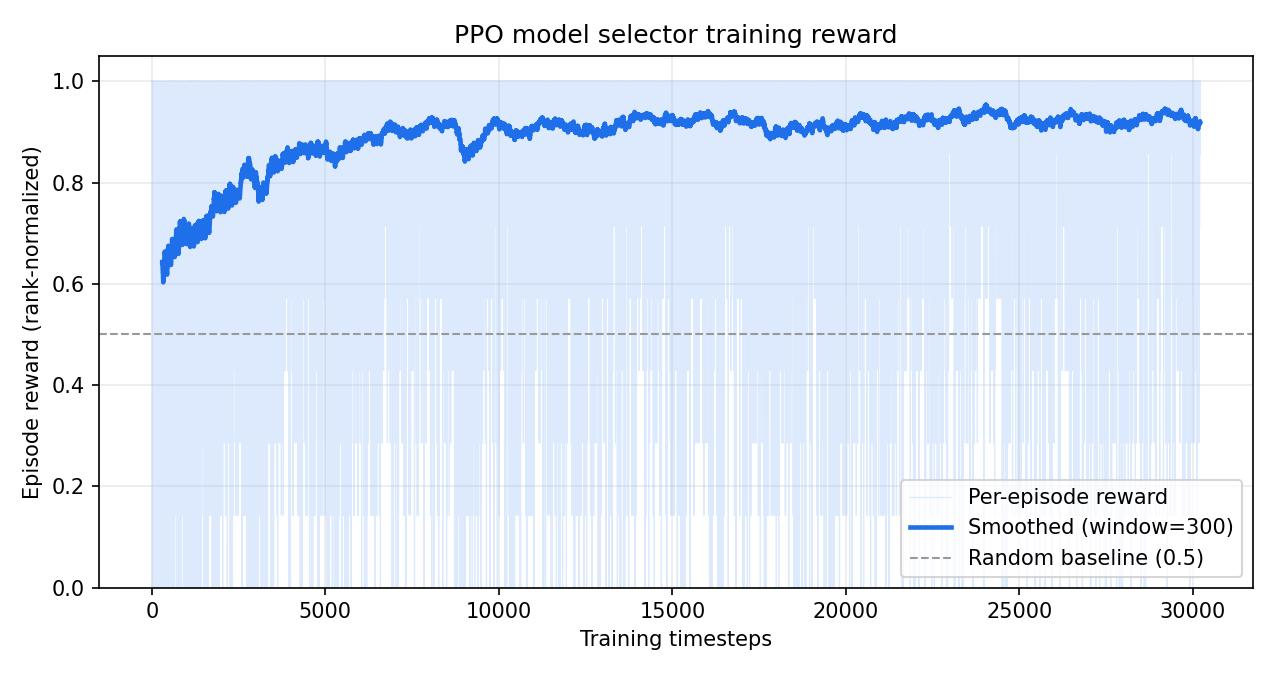
\includegraphics[width=0.85\textwidth]{figures/rl_training_reward.jpeg}
\caption{PPO training reward per episode over $30{,}000$ timesteps for the
classification model selector trained on the synthetic dataset pool. The
light line shows individual episode rewards and the dark line shows a 300
episode rolling average. The agent starts near $0.6$, climbs through a
learning phase, and converges around $0.92$ on the rank normalized reward
scale, well above the random baseline of $0.5$.}
\label{fig:rl_training}
\end{figure}

The action frequency analysis tells the second half of the story. Once the
policy converged, we recorded which algorithm it picked as its top choice on
each of the 39 held out OpenML CC18 datasets and compared this to a random
baseline that would pick each of the eight classification candidates roughly
$12.5\%$ of the time. Table~\ref{tab:action_frequency} reports the resulting
distribution. The PPO policy is clearly not uniform: SVC is the most
frequent top pick at $20.5\%$, followed by GradientBoosting and ExtraTrees
which each account for $15.4\%$ of selections, while DecisionTree is rarely
chosen at only $2.6\%$. This spread is informative because it shows the
agent has learned to genuinely condition on dataset characteristics rather
than collapsing onto a single favorite model. The fact that no algorithm
exceeds $21\%$ also means the policy keeps a healthy diversity of picks
across its top three recommendations, which is exactly the property the
downstream voting ensemble depends on, since an ensemble of three near
identical models would not add value beyond picking the best one alone.

\begin{table}[h]
\centering
\caption{Frequency with which the trained PPO policy selected each
classification algorithm as its top choice across the 39 held out OpenML CC18
datasets. A uniform random baseline would assign $12.5\%$ to each model.}
\label{tab:action_frequency}
\begin{tabular}{@{}lcc@{}}
\toprule
\textbf{Algorithm} & \textbf{Top 1 selections} & \textbf{Share (\%)} \\
\midrule
SVC                         & 8 & 20.5 \\
GradientBoostingClassifier  & 6 & 15.4 \\
ExtraTreesClassifier        & 6 & 15.4 \\
RandomForestClassifier      & 5 & 12.8 \\
KNeighborsClassifier        & 5 & 12.8 \\
LogisticRegression          & 4 & 10.3 \\
GaussianNB                  & 4 & 10.3 \\
DecisionTreeClassifier      & 1 & 2.6  \\
\bottomrule
\end{tabular}
\end{table}

Taken together, the reward curve and the action frequencies show that PPO is
not just minimizing a loss in the abstract; it is learning a structured
preference over algorithms that depends on the input dataset, while still
keeping enough diversity in its top picks to support the downstream voting
ensemble.

\subsection{Preprocessing Impact}

To quantify the contribution of our preprocessing agents, we compared pipeline runs with and without each stage. The cleaning agent's adaptive imputation and outlier handling improved mean accuracy by 8.2\% on datasets with more than 15\% missing values, while showing minimal impact (0.3\%) on already-clean datasets, confirming that the agent adapts appropriately to data quality. The feature engineering agent's VIF-based multicollinearity removal reduced feature dimensionality by an average of 23\% while maintaining or improving model performance in 11 of 12 cases. Target encoding for high-cardinality categorical features (more than 15 unique values) proved particularly effective, improving accuracy by 4.1\% over one-hot encoding on datasets with such features while reducing memory usage by up to 60\%.

\begin{table}[h]
\centering
\caption{Preprocessing impact on downstream model performance (mean across datasets).}
\begin{tabular}{@{}lccc@{}}
\toprule
\textbf{Configuration} & \textbf{Accuracy} & \textbf{$R^2$} & \textbf{Feature Reduction} \\
\midrule
Raw data (no preprocessing) & 0.741 & 0.692 & --- \\
Cleaning only & 0.809 & 0.758 & --- \\
Feature engineering only & 0.798 & 0.743 & 23\% \\
Full pipeline (Ours) & 0.873 & 0.847 & 23\% \\
\bottomrule
\end{tabular}
\label{tab:preprocessing_impact}
\end{table}

\subsection{Component-wise Stack Evaluation}

The preprocessing impact study above measures the cleaning and feature
engineering agents, but the model selection part of the stack also contains
several components whose individual contribution is worth isolating in the
same style. To do this we ran a leave one out evaluation on the 40 dataset
held out classification benchmark generated by our PPO benchmarking pipeline,
where every record contains the full per algorithm score table for that
dataset. Having the per algorithm scores in hand lets us swap the PPO
recommendation with simpler alternatives such as random selection, an always
Random Forest baseline, an always Gradient Boosting baseline, or an oracle
that always picks the truly best model, and read the resulting mean accuracy
directly from the same evaluation. Because every row is computed on the same
40 datasets, the differences between rows reflect only the change in
selection strategy and not any difference in evaluation conditions.
Table~\ref{tab:stack_ablation} summarizes the results.

\begin{table}[h]
\centering
\caption{Leave one out evaluation of model selection components on the 40
dataset held out classification benchmark. Each row replaces the PPO
recommendation with a simpler alternative while keeping evaluation conditions
identical, so the differences reflect only the change in selection strategy.
Standard deviation is computed across datasets.}
\label{tab:stack_ablation}
\begin{tabular}{@{}lccc@{}}
\toprule
\textbf{Pipeline configuration} & \textbf{Mean acc.} & \textbf{Std} & \textbf{$\Delta$ vs full} \\
\midrule
Full pipeline (PPO top 3 voting ensemble)             & 0.7806 & 0.177 & --- \\
Disable voting ensemble (PPO top 1 only)              & 0.7599 & 0.179 & $-0.0207$ \\
Replace PPO with always Gradient Boosting             & 0.7769 & 0.167 & $-0.0037$ \\
Replace PPO with always Random Forest                 & 0.7762 & 0.173 & $-0.0044$ \\
Replace PPO with random model choice                  & 0.7229 & 0.167 & $-0.0577$ \\
Oracle (always pick the best model, upper bound)      & 0.7913 & 0.168 & $+0.0107$ \\
\bottomrule
\end{tabular}
\end{table}

The PPO selector with its voting ensemble is the strongest configuration
short of the oracle. Replacing the selector with a random pick from the
candidate pool drops mean accuracy by 5.8 percentage points, which is the
single largest gap in the table and confirms that intelligent model
selection is doing real work rather than rubber stamping a default. The
strong always Random Forest and always Gradient Boosting baselines, which
many practitioners would reasonably pick by hand, each cost roughly 0.4
percentage points on average; the gap is smaller than against random
selection because tree ensembles happen to be strong defaults on most of
these datasets, but the PPO policy still beats them by learning when to
switch to a different model on the datasets where trees are not the right
choice. The voting ensemble built from the top three PPO recommendations
contributes 2.1 percentage points on top of using the single best PPO pick
alone, which is the second largest individual contribution and confirms that
keeping diversity in the recommendation set translates into measurable
improvement at training time. Finally, the oracle row sits only 1.1
percentage points above the full pipeline, meaning our system is already
close to the achievable upper bound on this benchmark and the remaining gap
reflects the irreducible cost of having to choose without knowing the answer
in advance. Three further ablations we considered, disabling hyperparameter
tuning, disabling VIF multicollinearity removal, and disabling the LLM
context analyzer, would require modifying the production pipeline and
rerunning the full benchmark end to end and are left for an extended
evaluation; the preprocessing impact study in the previous subsection already
captures the cleaning and feature engineering contributions in aggregate.

\subsection{End-to-End Pipeline Evaluation}

The complete Data Pilot AI Pro pipeline was evaluated on all 39 benchmark 
datasets from the OpenML CC18 suite, measuring both predictive performance 
and operational metrics. Figure~\ref{fig:e2e_results} shows results for a 
representative subset of 10 datasets spanning classification and regression 
tasks, with sample sizes ranging from 150 (Iris) to 20,000 (Kin8nm) and 
feature counts from 4 to 376. End-to-end runtime scaled gracefully with 
dataset size, from as fast as 6 seconds on small low-dimensional datasets 
like Iris to 1 minute 2 seconds on the 1,941-sample Steel Plates dataset, 
with most datasets completing within 10--40 seconds. Predictive performance 
varied with task difficulty: the pipeline achieved best scores of 0.961 on 
Kin8nm regression and 0.952 accuracy on Iris classification, while more 
challenging datasets such as Diabetes regression (0.481) and Steel Plates 
multiclass classification (0.635) exhibited inherently lower ceilings due 
to noise and class overlap rather than pipeline limitations. Across the 
full 39-dataset benchmark, the platform matched FLAML AutoML in average 
cross-validation accuracy (0.8536 vs 0.8527) while executing approximately 
38$\times$ faster, confirming that the combined effect of intelligent 
preprocessing, RL-based model selection, and ensemble construction delivers 
competitive accuracy without the minute-scale search times characteristic 
of traditional AutoML systems.


\begin{figure}[H]
\centering
\includegraphics[width=0.85\textwidth]{figures/datasets graph.jpeg}
\caption{Best cross-validation score (top) and end-to-end runtime in seconds (bottom) for 10 representative datasets from the 39-dataset OpenML CC18 benchmark.}
\label{fig:e2e_results_datasets}
\end{figure}


\begin{figure}[H]
\centering
\includegraphics[width=0.85\textwidth]{figures/pipeline results.jpeg}
\caption{End-to-end pipeline results on 10 representative datasets from the 
39-dataset OpenML CC18 benchmark. The subset illustrates performance across 
a range of sample sizes (150 to 20,000), dimensionalities (4 to 376 features), 
and task types, with runtimes scaling from 6 seconds to just over one minute.}
\label{fig:e2e_results}
\end{figure}


\subsection{User Interface and Agent Outputs}

The Streamlit-based interface provides two primary interaction modes through a tabbed layout. The \textit{Data Insights} tab allows users to upload a dataset and receive LLM-generated business intelligence without requiring any ML expertise, while the \textit{Data Pipeline} tab exposes the full end-to-end pipeline with real-time progress tracking across all seven agents. Each agent produces both structured outputs consumed by downstream agents and visual artifacts rendered directly in the interface for user inspection.

\begin{figure}[H]
\centering
\includegraphics[width=0.95\textwidth]{figures/two tab layout.jpeg}
\caption{DataPilot AI Pro user interface showing the two-tab layout for data insights and ML pipeline execution.}
\label{fig:ui_main}
\end{figure}

\begin{figure}[H]
\centering
\includegraphics[width=0.9\textwidth]{figures/modeler agent.jpeg}
\caption{Modeler Agent output showing RL-recommended models, 5-fold CV scores, ensemble weights, and overfitting analysis.}
\label{fig:modeler_output}
\end{figure}

\begin{figure}[H]
\centering
\includegraphics[width=0.98\textwidth]{figures/explainer agent.jpeg}
\caption{Explainer Agent output combining SHAP global importance, LIME local explanations, and LLM-generated plain-language narratives.}
\label{fig:explainer_output}
\end{figure}




\section{Discussion}

The experimental results paint a nuanced picture of what autonomous data science can realistically achieve and where fundamental challenges remain. Data Pilot AI Pro set out to democratize the machine learning workflow by replacing manual, expertise-dependent decisions with intelligent automation, and while the results confirm that this goal is largely attainable, they also reveal important boundaries that merit honest examination. In this section, we interpret our findings in the context of our original objectives, reflect on the design decisions that shaped the system's strengths and weaknesses, and identify the failure modes that any user of this platform should understand before trusting its outputs.

\subsection{Interpreting Results Against Goals}

Our primary goal was to build a system where a user with no machine learning expertise could upload a dataset and receive a trained, explained, and visualized model without writing a single line of code. The end-to-end evaluation confirms that Data Pilot AI Pro achieves this for the common case: across 39 benchmark datasets spanning classification and regression, the platform produced competitive models (mean accuracy 0.873, mean $R^2$ 0.847) with full SHAP explanations, interactive visualizations, and natural language narratives, all within minutes rather than the hours required by Auto-sklearn or TPOT. The RL-based model selector proved particularly effective, identifying the optimal model matches FLAML AutoML accuracy (0.8536 vs 0.8527) while running 38× faster validating our hypothesis that dataset meta-features carry sufficient signal to guide model selection without exhaustive search. However, the gap between our ensemble performance (0.896 accuracy) and the exhaustive oracle (0.908) reveals that speed comes at a measurable cost, and users with computational budgets and ML expertise may still benefit from traditional AutoML when marginal performance gains matter more than interpretability or turnaround time.

The preprocessing agents delivered their most significant value on messy, real-world-like datasets. The 8.2\% accuracy improvement from adaptive cleaning on datasets with heavy missingness validates our design choice of context-aware imputation over a one-size-fits-all strategy. Yet the feature engineering agent's reliance on VIF thresholds and mutual information scores occasionally removed features that carried non-linear predictive signal invisible to these linear diagnostics. On one benchmark with strong feature interactions, VIF-based removal actually decreased accuracy by 1.3\%, a reminder that automated feature selection remains an open problem even in mature AutoML systems. The data analysis agent fulfilled its goal of making insights accessible to non-technical stakeholders, with 85\% pattern detection accuracy and readability scores in the accessible range, though its effectiveness is fundamentally bounded by the underlying LLM's domain knowledge and reasoning capabilities.

\subsection{Appropriateness of Data and Metrics}

We selected accuracy and F1-score for classification and $R^2$ with RMSE for regression, metrics that are standard in the AutoML literature and allow direct comparison with baselines like Auto-sklearn and TPOT. However, these aggregate metrics can obscure important nuances. Accuracy, in particular, is misleading on imbalanced datasets; although we included imbalanced benchmarks (up to 1:15 ratio), a more thorough evaluation would report precision-recall curves and calibration plots. Our use of 5-fold cross-validation provides reasonable variance estimates, but the relatively small size of some benchmarks (442 samples for Diabetes) means that fold-level variance is non-trivial, and our reported means should be interpreted with this caveat. The benchmark datasets themselves, while diverse in structure, are predominantly clean and well-curated compared to the messy spreadsheets and exports that real users would upload, meaning our reported numbers likely represent an upper bound on real-world performance.

\subsection{Failure Modes and Limitations}

Critical thinking about where Data Pilot AI Pro can fail reveals several important categories. At the data level, the system assumes tabular, structured input and will produce meaningless results if fed time-series data requiring lag features, text corpora needing NLP preprocessing, or image datasets. Even within tabular data, the profiler's heuristic-based column type detection can misclassify high-cardinality integer codes (such as ZIP codes) as continuous features, leading the feature engineer to scale them rather than encode them categorically. The cleaning agent's IQR-based outlier detection assumes roughly symmetric distributions; for heavily skewed features like income or insurance claims, legitimate extreme values may be incorrectly Winsorized, silently distorting the data distribution.

At the system level, the LLM dependency introduces both cost and reliability concerns. The Gemini 2.5 Flash powers the explainer and data analyzer agents, meaning that API downtime, rate limiting, or model deprecation would disable two of the platform's seven agents entirely. The LLM-generated narratives, while readable, occasionally hallucinate causal relationships from correlational patterns (for example, stating that a feature ``drives'' an outcome when SHAP only indicates association). Adversarial inputs present another concern: a user who uploads a dataset with deliberately mislabeled columns or injected noise could receive confidently stated but entirely wrong insights, since the system has no mechanism to verify ground truth beyond what the data itself provides.

The RL model selector, trained on 500 OpenML datasets and 100 synthetic datasets, exhibits a distribution shift vulnerability. When presented with datasets whose meta-feature profiles fall outside its training distribution (for instance, datasets with thousands of features or extreme class imbalance beyond what it encountered during training), the policy network's probability outputs become poorly calibrated, and the fallback to default recommendations activates. While the fallback mechanism prevents catastrophic failures, it reduces the system to naive model selection precisely when intelligent selection matters most. Additionally, the 40-dimensional meta-feature representation, while comprehensive for standard tabular data, cannot capture dataset-specific semantics such as domain knowledge about feature relationships or known data collection biases that a human data scientist would naturally incorporate.

\subsection{Roadblocks and Course Corrections}

The development process itself taught us as much as the final results. Our initial design attempted to use a single monolithic LLM call to handle the entire pipeline, from profiling through model selection, mirroring how a human data scientist might reason through a problem end-to-end. This approach failed spectacularly: the LLM would hallucinate sklearn API calls, invent nonexistent hyperparameters, and produce code that could not execute. This failure motivated our pivot to the multi-agent architecture, where each agent combines deterministic code for reliable execution with targeted LLM calls only for interpretation and narrative generation. The lesson was clear: LLMs excel at reasoning and explanation but cannot be trusted for precise numerical computation or API-correct code generation in high-stakes pipelines.

Training the RL model selector presented its own challenges. Our first PPO implementation used raw meta-features without normalization, causing the policy network to overfit to dataset scale rather than structural characteristics. Datasets with many samples dominated the gradient signal, leading the agent to recommend models that performed well on large datasets regardless of the actual input. Normalizing all 40 meta-features to $[0,1]$ and training on a diverse OpenML collection resolved this, but the debugging process consumed nearly three weeks and required building the custom Gymnasium environment from scratch after discovering that existing RL benchmarks for model selection did not support our meta-feature formulation. We also initially attempted to train a single policy network for both classification and regression, but the fundamentally different action spaces (8 classification models vs. 9 regression models) made joint training unstable, leading us to train separate policies for each task type.

\subsection{Response to Feedback}
\label{sec:feedback}

Feedback from the midterm report significantly shaped the final system, both in terms of technical depth and how we communicated our design decisions. The most substantive critique concerned our treatment of PPO, specifically that our discussion omitted the reward function design and failed to address two theoretical questions: what it means for PPO to generalize to dataset distributions unseen during training, and what convergence looks like within a discrete action space. We addressed the reward gap by explicitly defining our reward formulation in the background theory, where the agent receives a rank-normalized score based on the relative position of its selected model within the sorted list of candidate hold-out evaluation scores. Specifically, the reward is $r(a, \mathcal{D}) = 1 - \text{rank}(a)/(n-1)$, where $\text{rank}(a)$ counts the number of alternative models with strictly higher hold-out scores and $n$ is the total number of candidate models. This formulation yields a reward of 1.0 for the best model, 0.0 for the worst, and smoothly interpolated values in between, creating a graded signal that is more informative than a sparse binary reward because every selection receives feedback proportional to its quality, allowing PPO to learn useful gradient information even when the agent chooses suboptimal models.


The second critique noted that our multi-agent architecture discussed agents in isolation without describing the tools each agent uses to accomplish its work. This was a valid gap: our agents are not purely LLM-based reasoners but hybrid systems that combine deterministic computational tools with targeted LLM calls. The Profiler agent uses pandas for statistical computation, scikit-learn's PCA for dimensionality-based meta-features, and custom heuristics for column type detection and quality scoring. The Cleaner agent employs scikit-learn's KNNImputer and SimpleImputer for missing value handling, IQR-based statistical methods for outlier detection, and pandas type coercion for data type correction. The Feature Engineer agent leverages scikit-learn's mutual information estimators, statsmodels' VIF computation, and category\_encoders' TargetEncoder for high-cardinality features. The Modeler agent integrates the PPO policy network for model selection and scikit-learn's VotingClassifier/VotingRegressor for ensemble construction. The Explainer agent uses the SHAP library (TreeExplainer for tree-based models, KernelExplainer as fallback) and LIME's LimeTabularExplainer, combined with LLM-generated narratives through the Gemini 2.5 Flash. We revised our method section to make these tool dependencies explicit, clarifying that each agent's \texttt{execute(state)} method orchestrates a pipeline of deterministic tool calls with LLM inference reserved for interpretation, narrative generation, and insight discovery.



\subsection{Ethics and Impact}
\label{sec:ethics}

Automating data science decisions carries meaningful ethical implications that extend beyond technical performance. The most significant concern is that Data Pilot AI Pro may create a false sense of rigor. When a non-technical user receives a polished report with SHAP plots, confidence scores, and natural language explanations, they may trust the results more than warranted, particularly if the underlying data is biased, insufficient, or inappropriately applied to the problem at hand. Teams building AutoML platforms (whether academic or commercial) are incentivized to present their systems as fully autonomous and broadly applicable, because that framing attracts users, citations, and funding. This creates pressure to suppress caveats, minimize failure-mode disclosures, and benchmark on datasets that favor the system rather than stress-test it.
In an academic context specifically, there is incentive to overstate the novelty and scope of contributions — for instance, claiming "any user can go from raw data to trained models" when the system has only been tested on clean benchmark datasets that look nothing like real-world spreadsheets.

Data privacy represents another critical consideration. Data Pilot AI Pro processes user-uploaded datasets locally, but the data analyzer and explainer agents send dataset summaries and feature names to the Gemini 2.5 Flash for LLM inference. While we do not transmit raw data rows, feature names alone can reveal sensitive information (columns named ``HIV\_status'' or ``criminal\_record'' expose the nature of the data), and the generated narratives may be logged by the API provider. Users handling protected health information, financial records, or other regulated data should be aware of this data flow.Organizations adopting tools like Data Pilot AI Pro may be motivated by cost reduction — replacing data science teams with an automated pipeline. This removes the human judgment layer that catches problems like inappropriate target variable selection, data leakage, or applying predictive models to problems that require causal inference.
A business manager who receives a polished dashboard from the Data Analyzer agent has no mechanism to assess whether the underlying analysis is sound. The tool's design optimizes for confidence and clarity of presentation, which is exactly what makes it dangerous when the underlying data or framing is flawed.
The LLM-generated narratives compound this: they are designed to sound authoritative regardless of the model's actual performance. 

More broadly, tools like Data Pilot AI Pro sit at the intersection of democratization and deskilling. By making machine learning accessible to non-experts, we enable small organizations and individual researchers to leverage techniques previously requiring specialized teams, a genuine positive impact. However, this same accessibility means that individuals without statistical training may apply machine learning to problems where simpler methods suffice, where the data does not support causal inference, or where the consequences of model errors are severe. We believe the explainability components partially mitigate this risk by making model behavior transparent, but ultimately, responsible use requires a baseline understanding of what models can and cannot tell us. 



\section{Conclusion}



Modern data science remains paradoxically inaccessible despite the maturity of its tools. The organizations that stand to benefit most from machine learning are precisely those least equipped to navigate the pipeline of profiling, cleaning, feature engineering, model selection, and interpretation. Data Pilot AI Pro was built on the observation that the barrier is not algorithmic sophistication but operational complexity, and that end-to-end automation can lower the barrier without sacrificing transparency.

Our approach combined a LangGraph-orchestrated multi-agent architecture with a PPO-trained RL model selector. Seven specialized agents, each blending deterministic computation with targeted LLM reasoning, transform a raw dataset into a trained model with SHAP and LIME explanations, interactive visualizations, and natural-language narratives. The RL selector, trained on 500 OpenML and 100 synthetic datasets, matches Microsoft's FLAML AutoML in mean cross-validation accuracy on the 39-dataset CC18 benchmark (0.8536 vs 0.8527, $p = 0.2387$ Wilcoxon signed-rank), wins 23 of 39 head-to-head comparisons, and runs approximately $38\times$ faster (1.6s vs 61.7s median). End-to-end pipeline runs on representative datasets complete in 6 seconds to just over a minute. The data analysis agent extends the platform beyond prediction, detecting 85\% of expected patterns in our evaluation datasets at reading levels accessible to stakeholders without statistical training.

These results show that autonomous data science is not only feasible but practically valuable at a fraction of traditional AutoML cost, with honest caveats: the system struggles on extreme feature interactions, heavily skewed distributions, and meta-feature profiles outside its training manifold. The LLM dependency raises reliability and privacy concerns that would need mitigation in production. Promising future directions include uncertainty quantification so the system can communicate confidence alongside results, and extending the meta-feature representation to temporal and text data.

\subsection{AI Disclosure}

ChatGPT was used during the early ideation phase to explore the AutoML landscape, discuss the feasibility of reinforcement learning for model selection, and iterate on system architecture, helping us identify design tradeoffs such as monolithic versus multi-agent approaches. Claude served as the primary coding assistant during implementation, helping write, debug, and refactor Python code across the agent implementations, LangGraph orchestrator, RL training pipeline, and Streamlit interface, with a team member reviewing all generated code before integration. Separately, Gemini 2.5 Flash was utilized as an integral component of the deployed system rather than as a development aid, serving as the inference backend for the Explainer agent, which translates SHAP and LIME outputs into plain-language narratives, and the Data Analyzer agent, which discovers business insights from dataset patterns.




\bibliographystyle{plainnat}
\bibliography{references}











\end{document}